\chapter{Costing}
\writer{Henri Videau}{6}
\section{Introduction}
In this chapter an updated costing of ILD is presented, corresponding to the latest design and dimensions of the detector. The method is very similar to that used in the costing exercise of the DBD, with two notable differences. Two size options are now costed: the large model IDR-L, very similar to the DBD baseline, and the small model IDR-S where the outer radius of the TPC has been reduced by about 30cm. In addition, the required manpower is now included in the costs, with an attempt to identify the in-kind laboratory manpower necessary to assemble the detector. 

The costing can now benefit from the construction of significant technological prototypes of the main subdetectors (chapter 5), as well as from spin-off detectors starting to be built for e.g. HL-LHC. The cost difference of the two models combined with the differences observed in their relative performances (chapter 8) will allow a better evaluation of the impact of the detector size than the simple scaling laws shown in the DBD. 

\section{The method}
The DBD costing had been made in an "ILC currency", the ILCU, in an effort to have a costing coherent between ILD, SiD and the accelerator. This implied making translations from different currencies using exchange rates and in most cases "Purchase Power Parities" (PPP). At that time an ILCU was 0.97 Euros using PPP's. Within the current exercise Euros(2018) are used as currency unit. When originating from Japan, e.g. for silicon diode matrices, the prices in Euros were provided by the vendors. Extrapolation of the DBD estimates to the present is made by converting the DBD ILCU's to Euros(2013) using PPP's as was done at the time (0.97 Euros for 1 ILCU), and propagating the cost to 2018 using as inflation rate the evolution of manufactured products in Europe [note Berriaud], amounting to 3\% between 2013 and 2018, as shown in figure~\ref{price_index}. At the end the two costs are the same. 
%(\textit{figure Berriaud}).

\begin{figure}[h!]
\centering
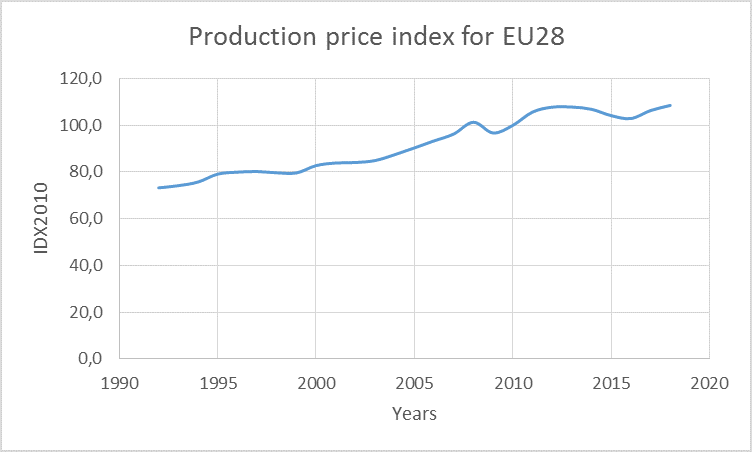
\includegraphics[width=1.0\hsize]{Costing/price_index.png}
\caption{Production price evolution over the 28 countries of UE.}
\label{price_index}
\end{figure}

Except for the currency the method used to establish the costing is totally similar to that of the DBD. It rests on the detailed knowledge of the fabrication processes and on the prices provided by the numerous prototypes built over the past years.  The idea is to identify the cost drivers, often very sensitive to strong price evolution, and to have a precise Work Breakdown System (WBS) identifying the procurements, the tooling, the fabrication operations. The WBS allows to estimate the manpower, which is now included in the costing. The manpower is twofold: in house laboratory  manpower mostly linked to the follow-up of the operations, but also to some construction work when high quality is required for small quantity items; industrial manpower which has to be estimated on top of the material costs in case no industrial offer is available for a given component.The manpower costs are converted into Euros(2018) assuming 80k Euros per FTE per Year as a mean unit cost over the different types of competences. The industrial manpower is incorporated into the material costs whereas the in house manpower is shown separately in order to allow an estimation of the in-kind contributions of the participating institutes. When the in house manpower is considered the cost appears as two numbers inside brackets, the first one is for material cost and the second for manpower.
It should be noticed that, except if specified, spares  are not included. More generally no contingency is applied.

\section{Subdetector costing}
The cost of each ILD subdetector is reviewed for both the large and the small ILD models. The inner and forward detectors which have the same configuration in both options (VTX, SIT, FTD, ECAL ring, VFS including LUMICAL, LHCAL, BEAMCAL) have only one quote, whereas others (TPC, ECAL, HCAL, COIL, YOKE and Iron Instrumentation) are costed for their two versions. 

The most expensive subdetector, the SIECAL, has received special attention in updating its costing of both material and manpower contributions, based on an updated detailed WBS. Some other subdetectors have fewer new pieces of information. For those which have only material costs available, the manpower costing has been estimated assuming the same manpower/material ratio as for the SIECAL. When no update is available versus the DBD version, the costing is propagated from the DBD estimate and simple scaling laws are used for the small version.

\subsection{VTX}
The Vertex Detector costing has been fully revisited [ref \textit{Note "ILD VXD and SIT Costing Estimates" by Marc and Auguste January 2019}] for its CMOS option based on recent detectors built for various experimental projects (see section 5.2.1). The results are summarised in  table~\ref{vertex_cost}.

%\textit{Check that manpower corresponds to in house only, in view of the size it is very likely}

\begin{table}\hspace*{-0cm}\small
\begin{tabular}[h!]{ l p{0.1\hsize}p{0.1\hsize}p{0.1\hsize} p{0.1\hsize}p{0.1\hsize}p{0.1\hsize} }
\toprule
\multicolumn{7}{ l }{{\bf Vertex detector}}\\
\midrule
Cost   & Sensors & Mechanics & Electronics & Services & Installation & Total \\
\midrule
Material    & 1.15   &  0.45   &  0.49    & 0.77 & 0.10 & 2.960 \\
Manpower    & 0.10   & 0.50    & 0.40     & 0.25 & 0.20 & 1.450 \\
\midrule
Total      & 1.25   &  0.95   &  0.89    & 1.02 & 0.30 & 4.410 \\
 \bottomrule
\end{tabular}
\caption{\label{vertex_cost}Elements of cost of the vertex detector (CMOS option) in MEuros.}
\end{table}

%\begin{figure}[h!]
%\centering
%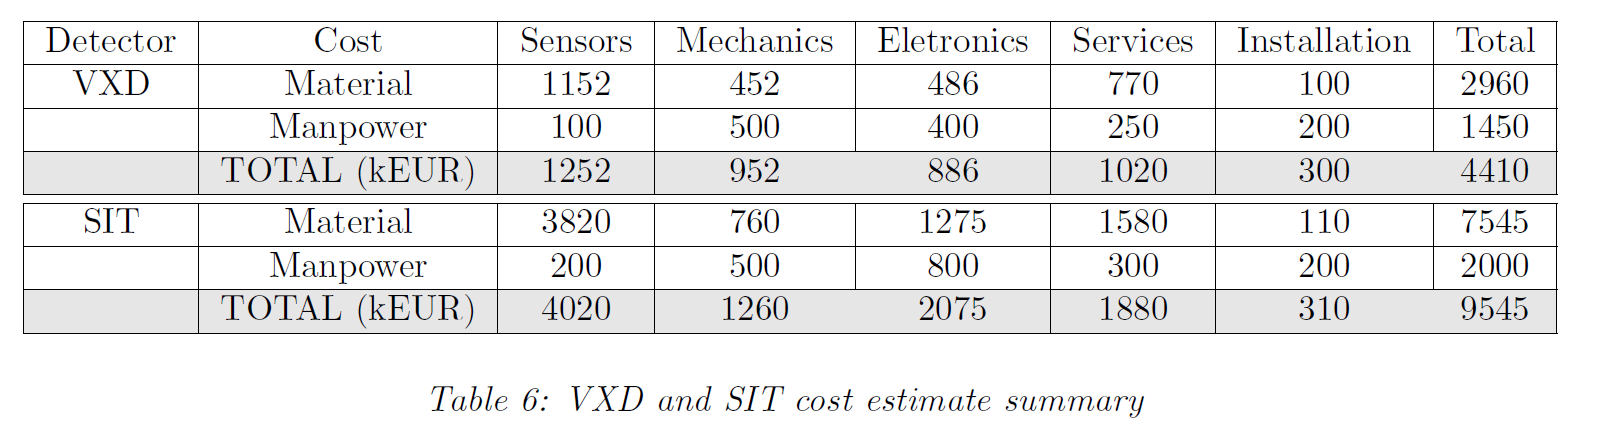
\includegraphics[width=1.0\hsize]{Costing/VXD_SIT.PNG}
%\caption{Contributions of the different items to the cost of the vertex detector.}
%\label{VXD_SIT}
%\end{figure}

\subsection{SIT}
In the simulation currently used for estimating the physics potential of the detector the SIT is made of strips like in the DBD. This version is costed, like the SET (see further) by extrapolation from the CMS tracker, it amounts to (0.8, 0.12) MEuros respectively for material and manpower. But the SIT costing has also been revisited in detail in a version based on CMOS pixels, a solution currently favoured. These new inputs are the same as used for the VTX costing [ref \textit{Note "ILD VXD and SIT Costing Estimates" by Marc and Auguste January 2019}]. The results are summarised in table~\ref{SIT_cost}. It can be noted that the pixel option is about ten times more expensive.

%\textit{Check that manpower corresponds to in house only}

Direct comparison to the DBD is not possible since the SIT was combined with the FTD in the DBD costing.

\begin{table}\hspace*{-0cm}\small 
\begin{tabular}[h!]{ l p{0.1\hsize}p{0.1\hsize}p{0.1\hsize} p{0.1\hsize}p{0.1\hsize}p{0.1\hsize} }
\toprule
\multicolumn{7}{ l }{{\bf Silicon Inner Tracking}}\\
\midrule
Cost   & Sensors & Mechanics & Electronics & Services & Installation & Total \\
\midrule
Material    & 3.82   &  0.76   & 1.28    & 1.58 & 0.11 & 7.55 \\
Manpower    & 0.20   & 0.50    & 0.80    & 0.30 & 0.20 & 2.00 \\
\midrule
Total      & 4.02   &  1.26   &  2.08    & 1.88 & 0.31 & 9.55 \\
\bottomrule
\end{tabular}
\caption{\label{SIT_cost}Elements of cost of the SIT (CMOS pixel option) in MEuros.}
\end{table}

\subsection{FTD}
There is no full update since the DBD. The current FTD configuration (chapter 5) includes 4 disks using pixel technology and 12 disks using strip technology. The cost of the pixel disks is estimated from the SIT pixel version, scaling with the area as (1.47, 0.4) Meuros. The cost of the strip disks is inferred from CMS to be (0.6, 0.09) MEuros. The global cost for the standard option is then of the order of (2.07, 0.5)MEuros. There is a tendency to  wish all disks to be made in pixels. This version can be roughly estimated from the SIT pixel version cost to be:(12.3, 3.3)MEuros.
% aires des disques: pixels 0.3 m² , strips 2.22, total 2.52
%du SET 0.25+0.04 du m². Soit strips 0.56 + 0.09
% La suface du SIT est 1.53 soit 4.9+1.3 du m²
%disques pixel 1.47 + 0.4  ou total 12.3 + 3.3
% donc modele classique 2.03 + 0.5
%mpdele pixel 12.3 +3.3
%\textit{How is this 2 Meuro estimated exactly?}

%\textit{Is there a chance to get a real update from Marcel Vos?}

\subsection{VFS and ECAL ring}

The three forward calorimeters, namely the BEAMCAL, the LUMICAL and the LHCAL, have been reexamined in detail in their new configuration with the new beam optics (chapter 5). The updated costing includes consideration of the mechanical elements, sensors, ASICs, front-end electronics, power supplies, data acquisition, tooling and manpower, separately for each of the subdetectors. Ancillary systems such as specific fanouts (for LUMICAL and LHCAL) and a laser positioning system needed for LUMICAL are also included. The resulting costs are summarised in the table~\ref{FCals_summary}. They correspond to a total of 8.44 MEuros and 6 FTE-years equivalent to 0.48MEuros.

%\textit{Trivial question: the costing is summing the 2 systems in both beam directions ?} 

The forward region also includes an ECAL ring making the transition from the LumiCal to the ECAL endcap. Its costing has been updated based on a rough extrapolation based on the silicon area from the SiECAL costing (see below). The ECAL rings silicon area is about  1\% of the full ECAL, barrel plus end-caps. The electronics is more similar to that of the LumiCal and the manpower is taken identical to that needed for the LumiCal.  The estimated cost of the two rings is then (1.5, 0.16) MEuros.  All the forward calorimetry, referred to as FCAL in the figure ~\ref{Costing:Large_cost_sharing}, is then estimated to (10, 0.64) Meuros.

%\begin{figure}[h!]
%\centering
%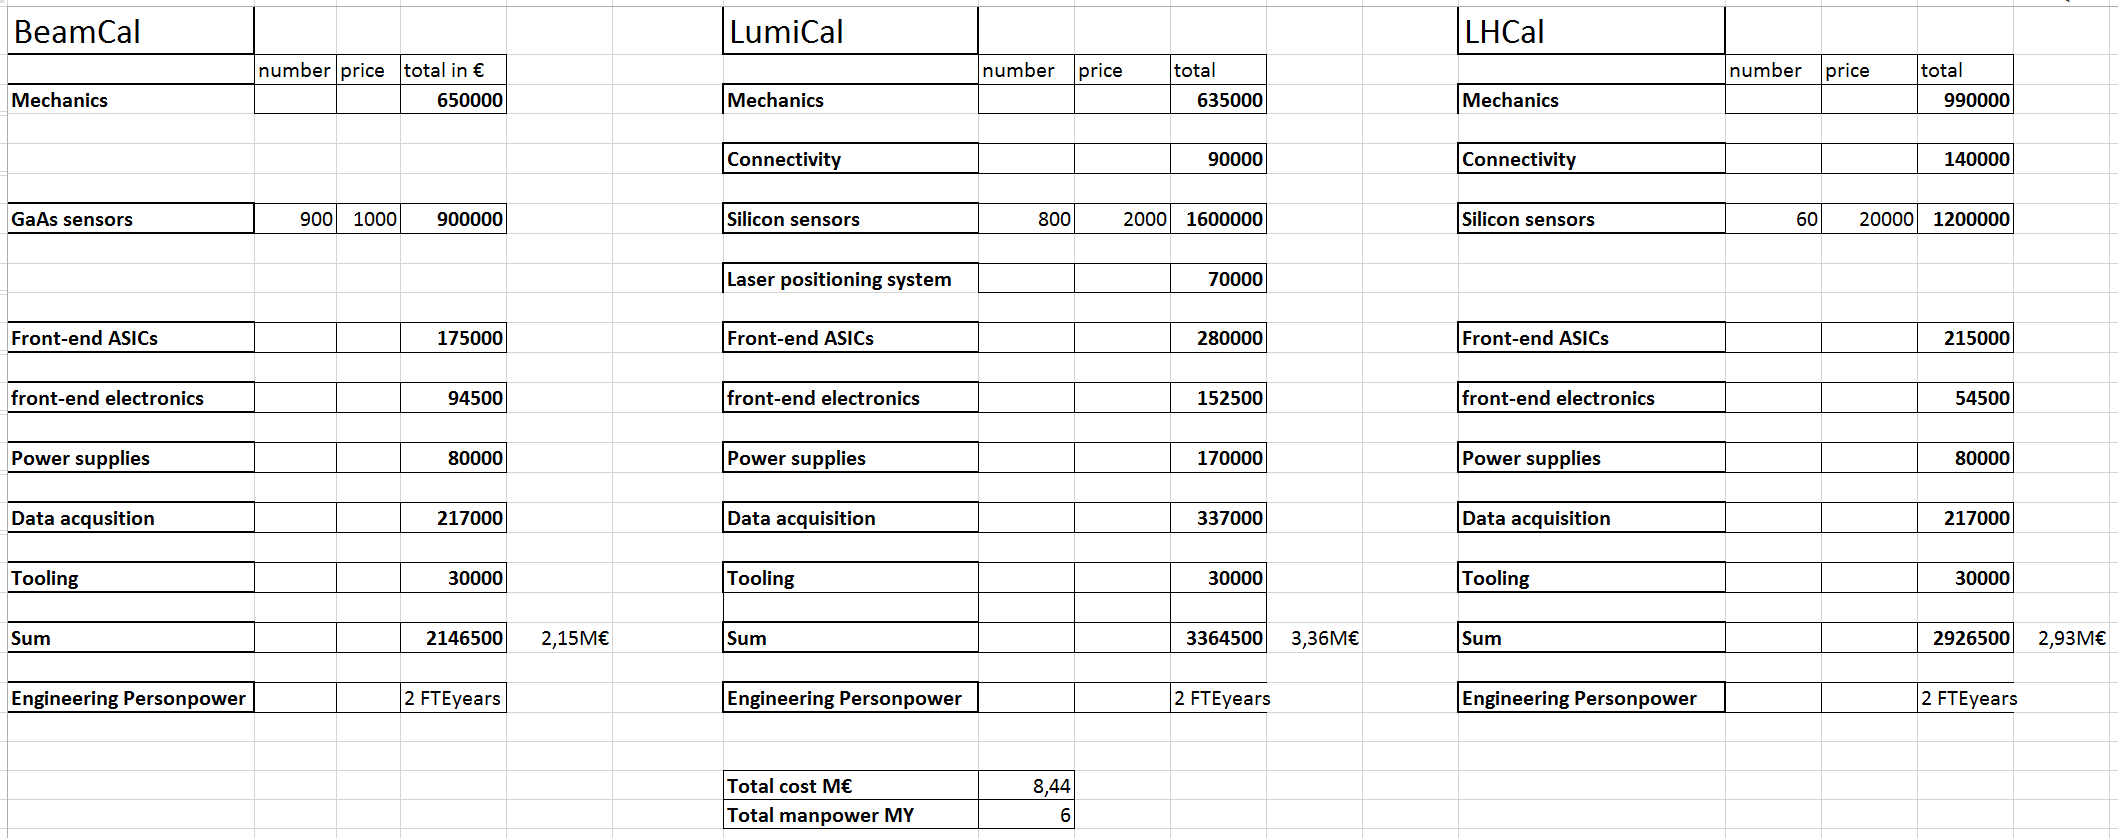
\includegraphics[width=1.\hsize]{Costing/Fcals_summary.PNG}
%\caption{Contributions of the different items to the cost of the forward calorimetry.}
%\label{Fcals_summary}
%\end{figure}

 \begin{table}\hspace*{-0cm}\small 
\begin{tabular}[h!]{ l p{0.2\hsize}p{0.2\hsize}p{0.2\hsize} }
\toprule
& BEAMCAL & LUMICAL & LHCAL \\
\midrule
Mechanics              & 0.65   & 0.64   & 0.99   \\
Connectivity           &        & 0.09   & 0.14   \\
Sensors                & 0.90   & 1.60   & 1.20  \\
Laser system           &        & 0.07   &       \\
Front-end ASICs        & 0.18   & 0.28   & 0.22   \\
Front-end electronics  & 0.10   & 0.15   & 0.05  \\
Power supplies         & 0.08   & 0.17   & 0.08    \\
Data acquisition       & 0.22   & 0.34   & 0.22  \\
Tooling                & 0.03   & 0.03   & 0.03   \\
\midrule
Total                  & 2.15  & 3.37   & 2.93  \\
\midrule
Manpower (FTE x Year)  &2       &2       & 2 \\
\bottomrule
\end{tabular}
\caption{\label{FCals_summary}Elements of cost of the forward calorimeters in MEuros and manpower in FTE x Year.}
\end{table}

\subsection{TPC}
There is no update since the DBD, where the quoted TPC price was 35.9 MILCU. This translates to 36.6 MEuros of 2018 and corresponds to the large ILD option. Using simple scaling laws the TPC of the small option is estimated to 27.0 MEuros. 

\textit{ Any chance to get an update from Paul Colas?}
\textit{What about manpower ?}

\subsection{SET}
The end cap part of the external silicon tracker, coined ETD, is no longer part of the ILD design as it was in the DBD.

%The cost from the DBD is quoted 21 MILCU for both SET and ETD. A cost for the SET alone can be guessed from the areas but the number of layers is different; the SET area over the total is about 0.73 and its cost is then claimed to be 15.3 MILCU or 14.84 MEuros 2008, or about 15.5 MEuros 2018 after running the Euro. No cost was established for the small model. It could be scaled from the large with the ratio of the radii: 0.807, providing a cost of 12.6 MEuros.

An estimate of the barrel part (SET) can now most accurately be derived from the cost of the CMS tracker which is also made of double-layer silicon strips. The CMS tracker cost is about 275kCHF per $m^2$ of detector, including silicon and mechanics. The SET area in the large ILD model is about 52.9 $m^2$, resulting in an estimated cost of 14.5 MCHF for the sensors and mechanics. Adding 20\% for the miscellaneous components such as cooling, power supply and back-end electronics results in a total estimate of 14.5 x 1.20 x 0.89 = 15.5MEuros. This estimate, based on the CMS tracker, is coherent with a propagation of the DBD estimate to the surface of the barrel SET only. The in house manpower included in this cost is estimated to 1.6 MEuros.
Using a simple scaling law the small SET model is then estimated to (11.2, 1.3) MEuros for a surface of 42.7 $m^2$. 



\subsection{ECAL}
\subsubsection{Silicon option (SiECAL)}
The DBD SiECAL costing amounted to 157 MILCU, propagating to about the same amount in MEuros(2018), with about half of the cost corresponding to the silicon diode matrices, and excluding manpower.

The updated costing of the SIECAL is based on a very detailed WBS informed from the fabrication processes of the SIECAL technological prototypes (chapter 5). This WBS follows a detailed and chronological fabrication description with the procurements for the different operations, the needed tooling and the fabrication steps, including manpower and duration, under the constraint that none should have a duration longer than two years. Most of the tooling has been kept at the same cost for the different ILD size options, which is slightly at the advantage of the large model for comparison of the costings between the different sizes.

Apart for a slight tungsten cost rise, the main difference with the DBD estimate comes from the evolution of the diode matrices estimation. In the updated costing the offer to CMS for the HGCAL matrices is used. The resulting total SIECAL cost reaches 119 MEuros excluding manpower. The in house manpower has also been estimated to 131 FTE x Years, equivalent to 11 MEuros, which results in a total amount of 130 MEuros.

Using similar inputs the small SIECAL version is costed to 92 MEuros for material. Including 9 MEuros for manpower, the total cost is 101 MEuros. 
A version of the small SIECAL with a slightly coarser sampling has also been estimated. For this version the number of active layers is reduced from 30 to 26 (section 5.2.4.1). The motivation for such a configuration is dictated by technical reasons rather than cost, but it is worth noting that the impact of the reduced sampling on the energy resolution is expected to be compensated by an increase of the silicon thickness to 725 micrometers. The reduced sampling provides a further cost reduction to (81, 8) MEuros.  

The various global costings are summarised in table~\ref{ECal_summary}. A breakdown of the contributions of the main items to the cost is shown in Figure~\ref{fig:det:ECalsm_Si_cost_sharing} for the small model with the baseline 30-layers sampling. The silicon matrices cost still dominates the procurements, but other items such as tungsten, printed boards and ASICs also represent significant parts. The in house manpower is around 10\% of the cost.

\begin{table}\hspace*{-0cm}\small 
\begin{tabular}[h!]{ l p{0.2\hsize}p{0.2\hsize}p{0.2\hsize} }
\toprule
Version& Material & Manpower & Total \\
\midrule
Large model                       & 119   & 11    & 130   \\
Small model                       & 92    &  9    & 101   \\
Small model with reduced sampling & 81.   &  8    & 89  \\
\bottomrule
\end{tabular}
\caption{\label{ECal_summary}Estimates for the three versions of the SIECAL (MEuros).}
\end{table}

\begin{figure}[h!]
\centering
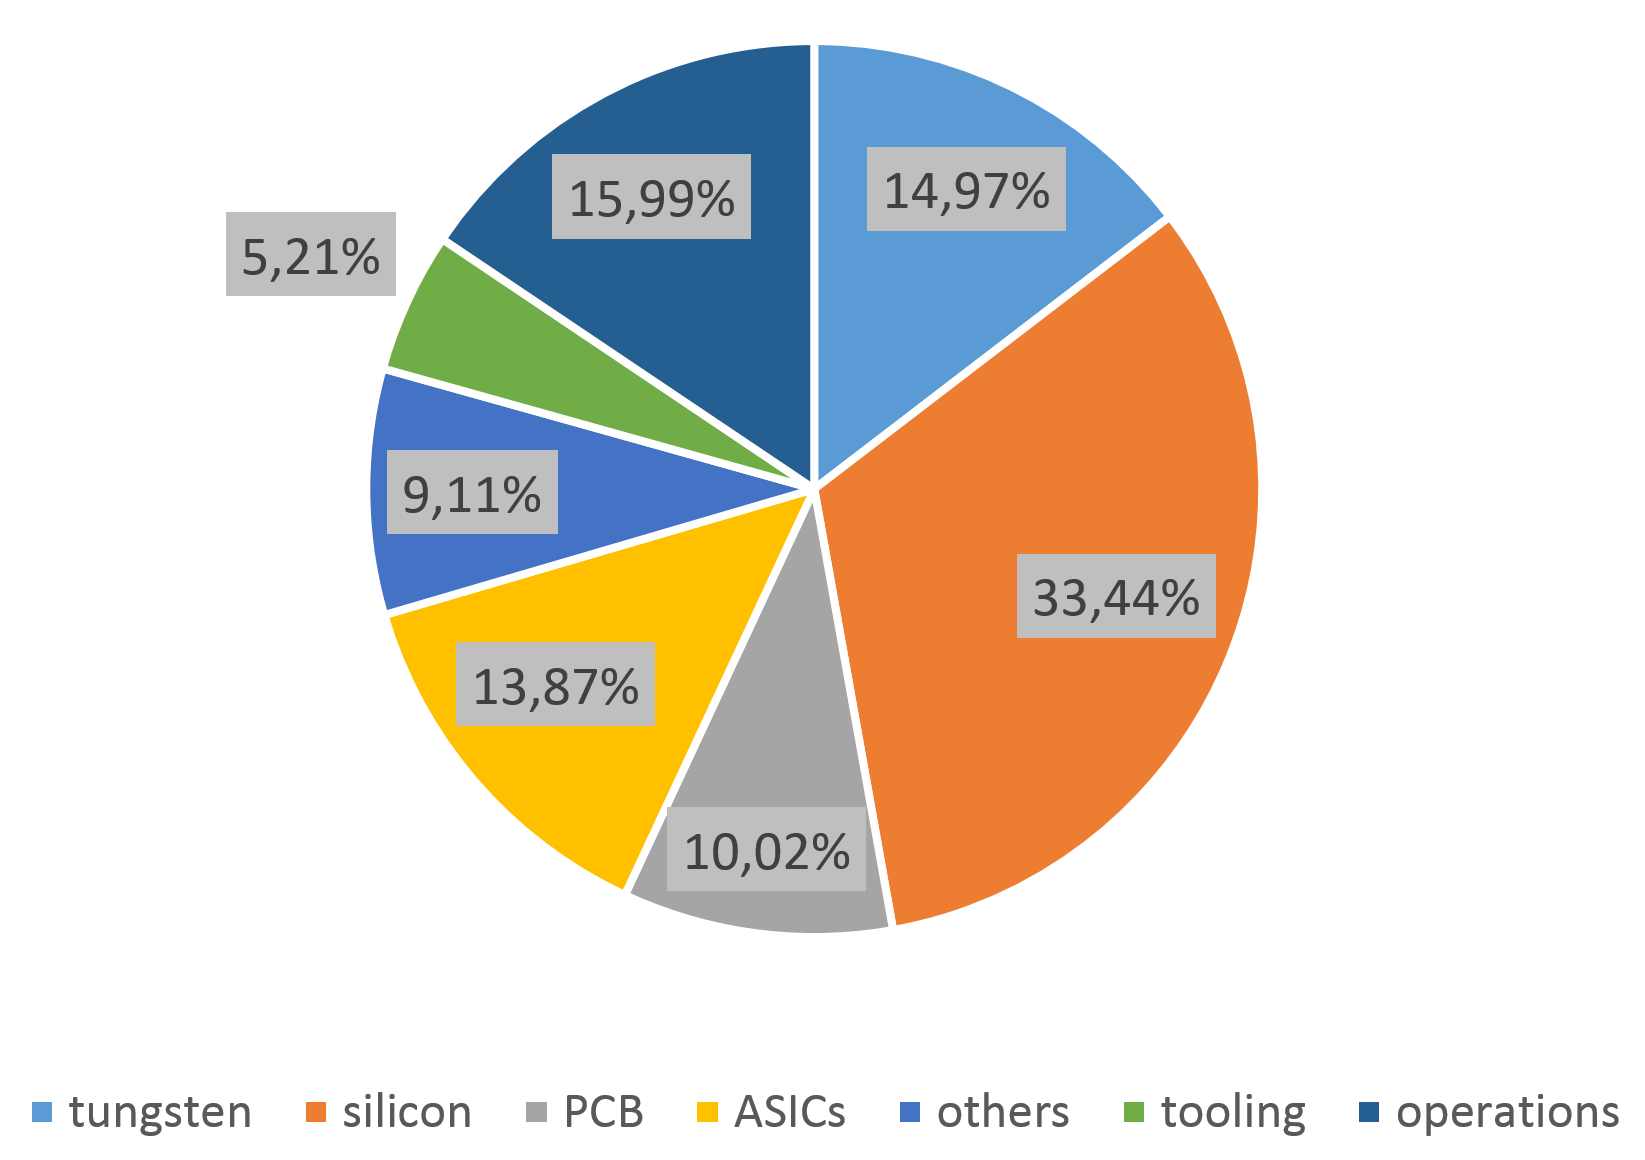
\includegraphics[width=0.8\hsize]{Costing/ECallg_Si_cost_sharing.PNG}
\caption{Contributions of the different items to the SIECAL cost in the case of the "large model".}
%\textit{The figure should be given for the baseline 30 layers sampling.}}
\label{fig:det:ECal26_Si_cost_sharing}
\end{figure}


\begin{figure}[h!]
\centering
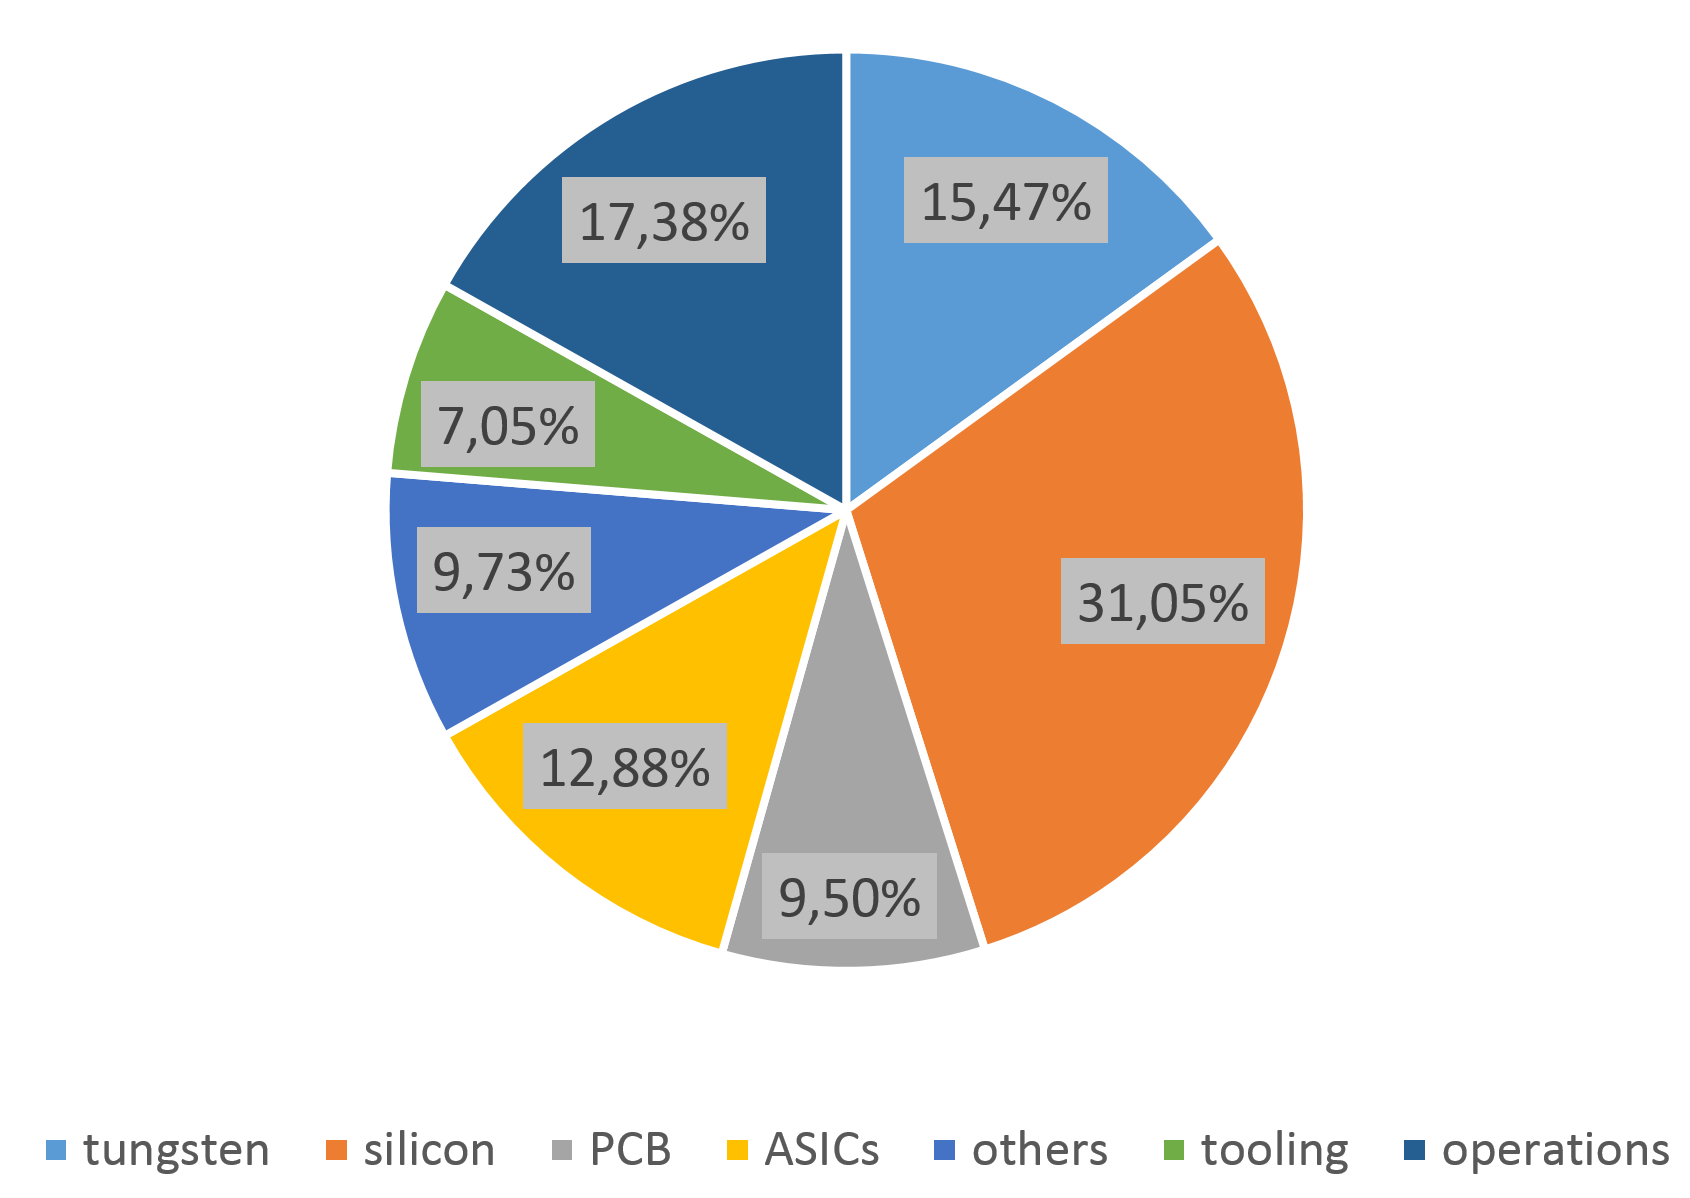
\includegraphics[width=0.8\hsize]{Costing/ECal26_Si_cost_sharing.PNG}
\caption{Contributions of the different items to the SIECAL cost in the case of the "small model" with a reduced sampling.}
%\textit{The figure should be given for the baseline 30 layers sampling.}}
\label{fig:det:ECal26_Si_cost_sharing}
\end{figure}

\begin{figure}[h!]
\centering
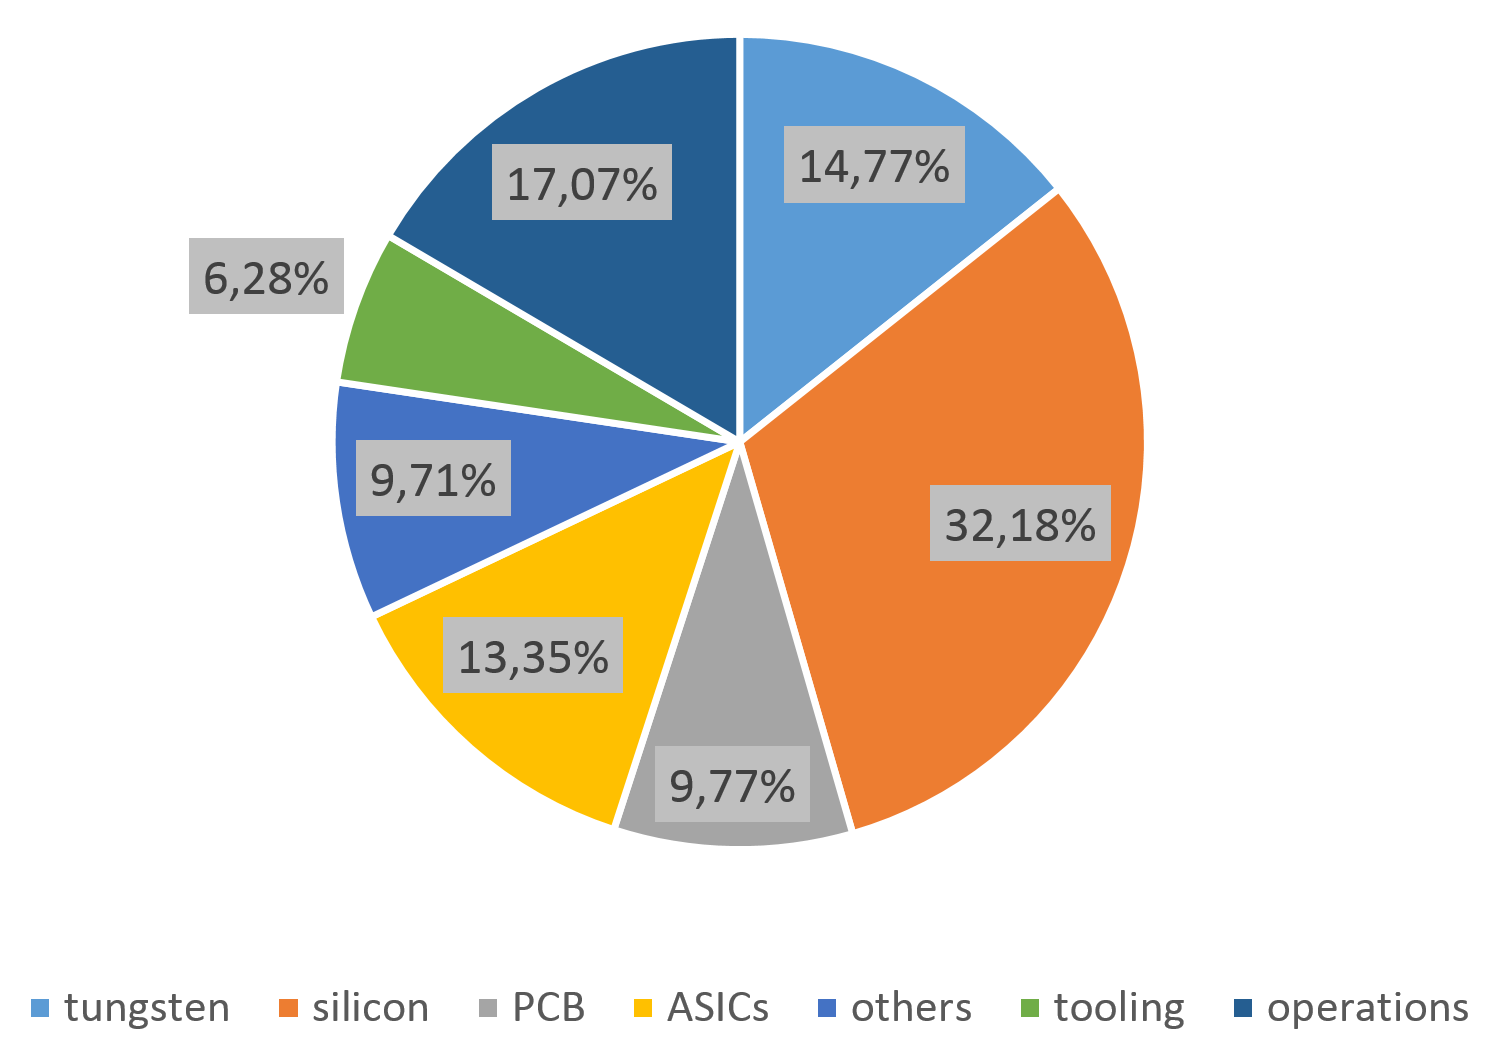
\includegraphics[width=0.8\hsize]{Costing/ECalsm_Si_cost_sharing.PNG}
\caption{Contributions of the different items to the SIECAL cost in the case of the "small model".} %\textit{The figure should be given for the baseline 30 layers sampling.}}
\label{fig:det:ECalsm_Si_cost_sharing}
\end{figure}

\subsubsection{Scintillator version (SCECAL)}
The SCECAL material costing from the DBD is considered to be still valid and amounted to 74 MILCU, propagating to 75 MEuros(2018), for the large ILD version. The in-house assembly manpower has since then been estimated to 11.5 MEuros. Applying simple scaling laws the SCECAL small version is costed to 62.5 MEuros for material and 9.5 MEuros for manpower.

\subsection{HCAL}
The costs proposed for the two versions are pretty close and for the cost summary will not be distinguished.
\subsubsection{Analog option (AHCAL)}
Since the DBD the application of the SiPM-on-tile technology to the CMS endcap calorimeter upgrade allows to consolidate the costing further. With about 400000 channels it represents an intermediate scale between the 22000 channel AHCAL prototype and the ILD AHCAL. 
The cost envelopes for the CMS SiPMs are consistent with the scaling assumed for ILD at the DBD times and so far confirmed in informal contacts with vendors. The AHCAL material costing from the DBD is therefore considered to be still valid. It amounted to 44.9 MILCU, propagating to 45.7 MEuros(2018), for the large ILD version. 
For the small model, a simple scaling corresponds to a factor 0.84 from the large to the small with a resulting material cost of 38.4 MEuros.

No detailed manpower cost estimate has been done. Assuming the same manpower/material ratio as for the SIECAL (9\%) the in-house assembly manpower is estimated to 4.1 MEuros for the large model and 3.5 MEuros for the small model.

\subsubsection{Semi-digital option (SDHCAL)}

The SDHCAL material costing from the DBD is considered to be still valid and amounted to 44.8 MILCU, propagating to 45.6 MEuros(2018), for the large ILD version. Applying simple scaling laws the SDHCAL small version is costed to 38.3 MEuros for material.

No detailed manpower cost estimate has been done. Assuming the same manpower/material ratio as for the SIECAL (9\%) the in-house assembly manpower is estimated to 4.1 MEuros for the large model and 3.4 MEuros for the small model.

\subsection{Magnet}
The costing of the magnet (coil and yoke) has been fully revisited [note Berriaud]. As for the DBD the anti-DID option (section 6.4) is not taken into account since its configuration is not fully defined. The main source of the current evaluation consists of the documentation of the CMS magnet, which has a similar size to that of ILD. When extrapolating to ILD the CHF costs from CMS have been converted into Euros at the exchange parity of the CMS magnet construction time, and the Euro inflation to 2018 taken into account. The resulting costs are summarised in table~\ref{magnet_cost}. One important change compared to the DBD estimation is the strong reduction in the yoke cost. At the time of the DBD a price of 6ILCU/kg had been agreed upon with SiD and CLIC, whereas the price payed for CMS corresponds to 3.5 Euros(2018)/kg. 

No attempt to cost the small ILD option has been made. A priori the cost of the small version is expected to be reduced. However the impact of the higher nominal field of 4T on the coil winding and on the flux return is not trivial and may counteract the reduced sizes. Keeping the small magnet cost similar to the large one may be a good approximation for the time being.

The magnet costing is likely to still evolve significantly in the future. For the coil industrial offers are expected from the Japanese companies which are currently studying it, including the anti-DID option. The yoke final cost will strongly depend on the final stray field constraints retained for ILD, as well as on the evolution of the iron market prices until ILD construction.

%\textit{Check iron cost used in chapter 6.4 to estimate yoke cost reductions given there for various options.}

\begin{table}\hspace*{-0cm}\small 
\begin{tabular}[h!]{ l p{0.2\hsize}  p{0.1\hsize} }
\toprule
%\multicolumn{7}{ l }{{\bf Silicon Inner Tracking}}\\
\textbf{Magnet system} & \textbf{88}\\
\midrule
\textbf{Coil} & \textbf{29.4}\\
\midrule
Conductor and winding & 18.5\\
Internal cryogenics and suspension &  3.7\\
Suspension system & 0.3 \\
Internal instrumentation & 0.9 \\
Tooling, assembling & 5.4 \\
Qualification and partial testing & 0.6\\
\midrule
\textbf{Ancillaries for coil} & \textbf{10.6}\\
\midrule
Cryogenics and vacuum & 6.5\\
Electrical power circuits & 0.9\\
Control and safety systems& 0.6 \\
Engineering (transport to cavern) & 2.1\\
Integration in cavern& 0.3 \\
Field mapping&0,3\\
\midrule
\textbf{Yoke and vacuum tank} & \textbf{48.4}\\
\midrule
Yoke steel including works and vacuum tank& 39.6\\
Support &1.2\\
Moving system& 2.6\\
Assembly& 4.8\\
Photogrammetry and survey& 0.3 \\
\bottomrule
\end{tabular}
\caption{\label{magnet_cost}Elements of cost of the magnet system in MEuros.}
\end{table}

%\begin{figure}[h!]
%\centering
%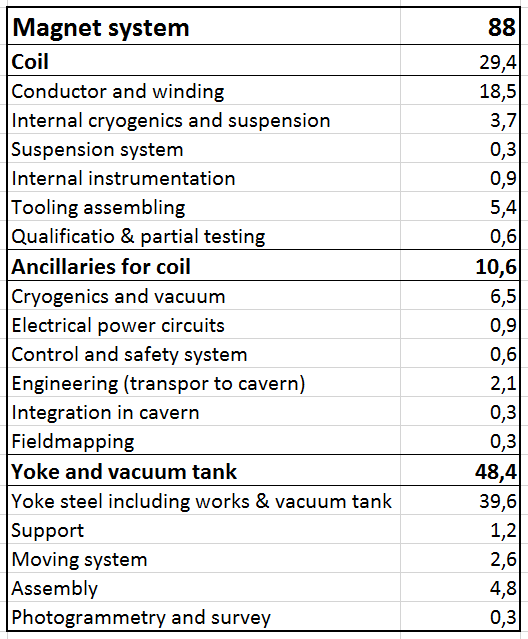
\includegraphics[width=0.5\hsize]{Detector/fig/Magnet_table.PNG}
%\caption{Magnet cost sharing. The costs are in MEuros}
%\label{fig:det:Magnet_cost_sharing}
%\end{figure}


\subsection{Iron instrumentation}
There is no update since the DBD, where the quoted iron instrumentation material cost was 6.5 MILCU for the 14 layers. This translates to 6.6 MEuros of 2018 and corresponds to the large ILD option. Using simple scaling laws the Iron instrumentation of the small option is estimated to 6.0 MEuros.

%\textit{For how many instrumented layers ?}

No assembly tooling and manpower has been estimated. Based on the SIECAL detector these contributions can be estimated to 0.6 MEuros for both the large and small options. 

\section{Global ILD costing.}
The subdetector costs presented in the preceding subsections are summarized in table~\ref{cost_summary} and summed up for the two ILD models.The global sum has been computed using the DBD solutions for SIT and FTD: SIT strips and FTD with 4 pixel disks and the rest with strips. It is obtained with the SiECal and AHCal versions in calorimetry but using the sDHCal makes no difference.
The inner system which offers no difference between the two sizes sums up to 15.8 + 2.7 = 18.5 for the "classical" solution and 32.8 + 7.4 = 40.2 for the favoured solution. The outer system sums up to 325.3 + 26.7 = 352.0 for the large model and 278.1 + 23.5 = 301.6  for the small one.
\begin{table}[h!]\hspace*{-0cm}\small
\begin{tabular}{ l p{0.2\hsize}p{0.1\hsize}p{0.2\hsize} p{0.2\hsize}p{0.1\hsize}}
\toprule
\bf {Item}& \bf {Large model} & \bf manpower&  \bf {Small model}&\bf manpower \\
\midrule
Inner part&&&&\\
Beam tube & 0.5 &  0.& idem&idem \\
VTX        & 2.96  &1.45  &  idem &idem \\
SIT strips & 0.8   &0.12 & idem&idem\\
SIT pixels & 7.55  &2.0 & idem&idem\\
FTD classic & 2.1   &0.5  & idem &idem  \\
FTD pixels  & 12.3  &3.3  & idem &idem  \\
LUMICAL & 3.37  & 0.16& idem&idem\\
ECAL ring & 1.5 & 0.16 & idem&idem\\
LHCAL   & 2.93  & 0.16&idem& idem\\
BEAMCAL & 2.15  & 0.16& idem&idem\\
%FCAL    & 9.95  & 0.64& idem&idem\\
\midrule
TPC & \it36.6 & 0 & \it27.0 & 0\\
%SET & 12.6& 1.9&10.8&1.7\\
SET    & 13.9& 1.6&11.2&1.3\\
SIECAL & 119 & 11.0 & 92. & 8.7\\
SCECAL & \it75 & 11.5 & \it62.5 & 9.5\\
AHCAL  & \it45.7 & 4.1 & \it38.4 & 3.5\\
SDHCAL & \it45.6 & 4.1 & \it38.3 & 3.4\\
Coil and ancillaries &  40 & 4& idem & idem\\
Yoke and vacuum tank &  48.4 & 5.2& idem & idem \\
Iron instrumentation  &  \it6.6 & 0.6 & 6 & 0.54\\
DAQ       & 1.1 & 0.16& idem& idem\\
Integration & 1.5 & 0 &idem&idem\\
Transportation& 12 & 0 & idem & idem \\
\midrule
Classical version & 341.1   &  29.4  & 303.1 & 26.5  \\
New version & 358.1   &  34.1  & 311.5 & 31.2  \\
\midrule
Total including MP classical     & 370.5   &    & 329.6 & 0  \\
Total including MP new     & 392.1   &    & 342.7 & 0  \\
 \bottomrule
\end{tabular}
\caption{\label{cost_summary}Global costing of ILD in MEuros. The numbers in italic are extrapolated from the DBD. The manpower has been translated from FTE-years to euros. The total sums use the classical solutions for SIT and FTD as well as the SIECAL and AHCAL cost estimates. 
%\textit{SET large cost does not sum to 15.5 ME as in text. }
%\textit{MP numbers should be revisited/completed along the method decribed in the text.} 
}
\end{table}

\section{Comparison to the DBD cost estimate.}
 The DBD ILD total cost amounted to 392MILCU, corresponding to ??? MEuros(2018). The relative sharing between the sub-detectors is shown for the different versions in the figures~\ref{fig:det:DBD_cost_sharing}, ~\ref{Costing:Large_cost_sharing}, ~\ref{Costing:Small_cost_sharing}. 
 
\begin{figure}[h!]
\centering
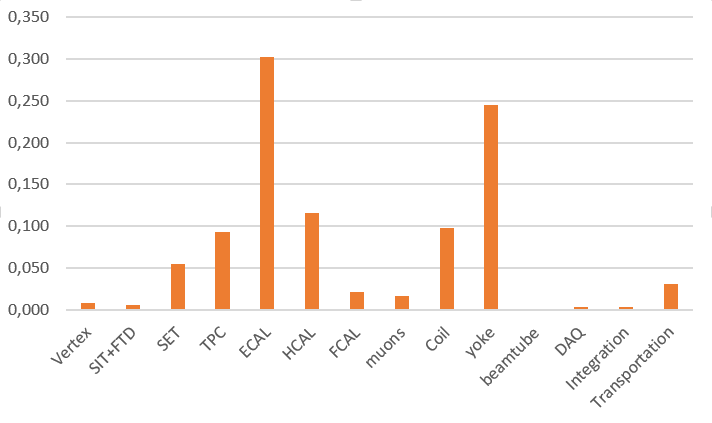
\includegraphics[width=0.8\hsize]{Detector/fig/DBD_cost_sharing.PNG}
\caption{ILD cost sharing as documented in the DBD}
\label{fig:det:DBD_cost_sharing}
\end{figure}

\begin{figure}[h!]
\centering
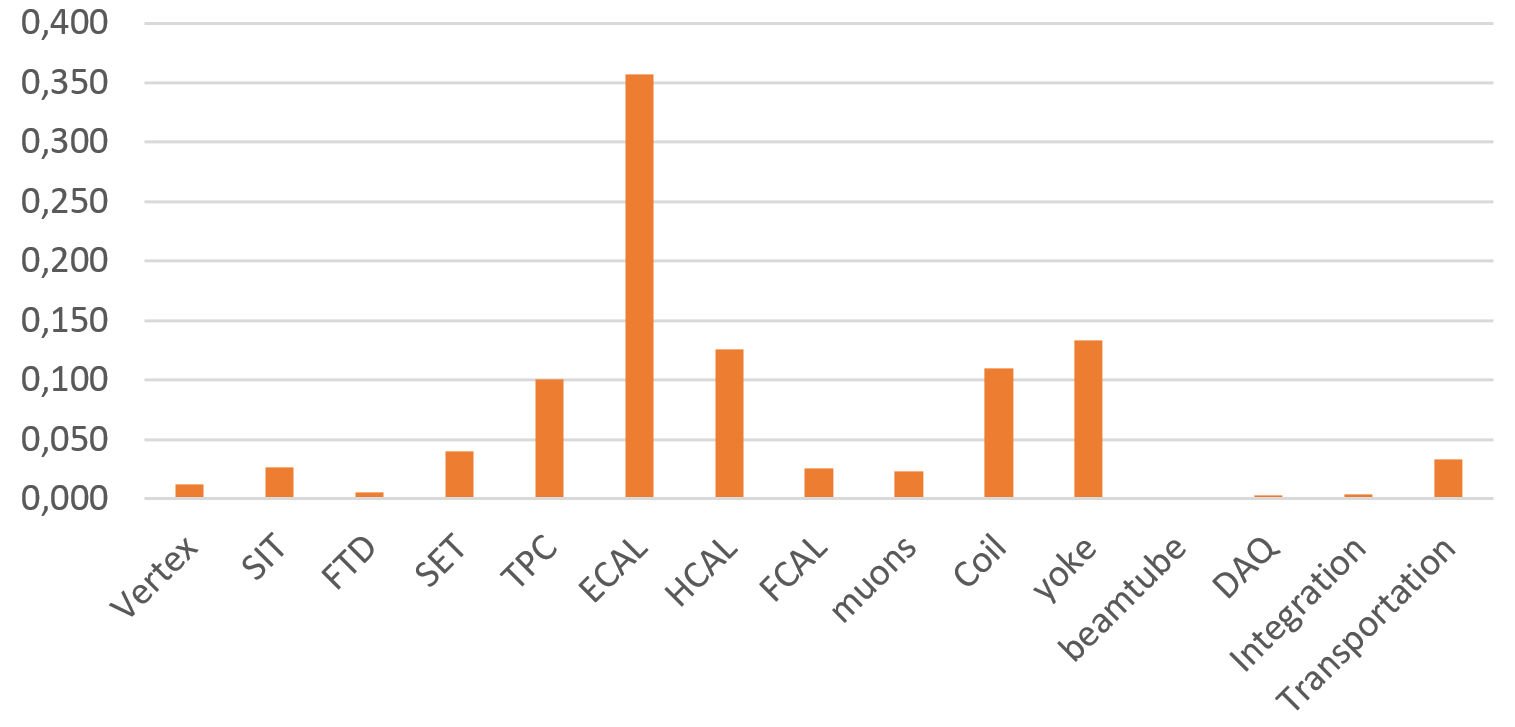
\includegraphics[width=0.8\hsize]{Costing/Large_cost_sharing.PNG}
\caption{ILD cost sharing in the large model. \textit{Empty FTD to be corrected.}}
\label{Costing:Large_cost_sharing}
\end{figure}

\begin{figure}[h!]
\centering
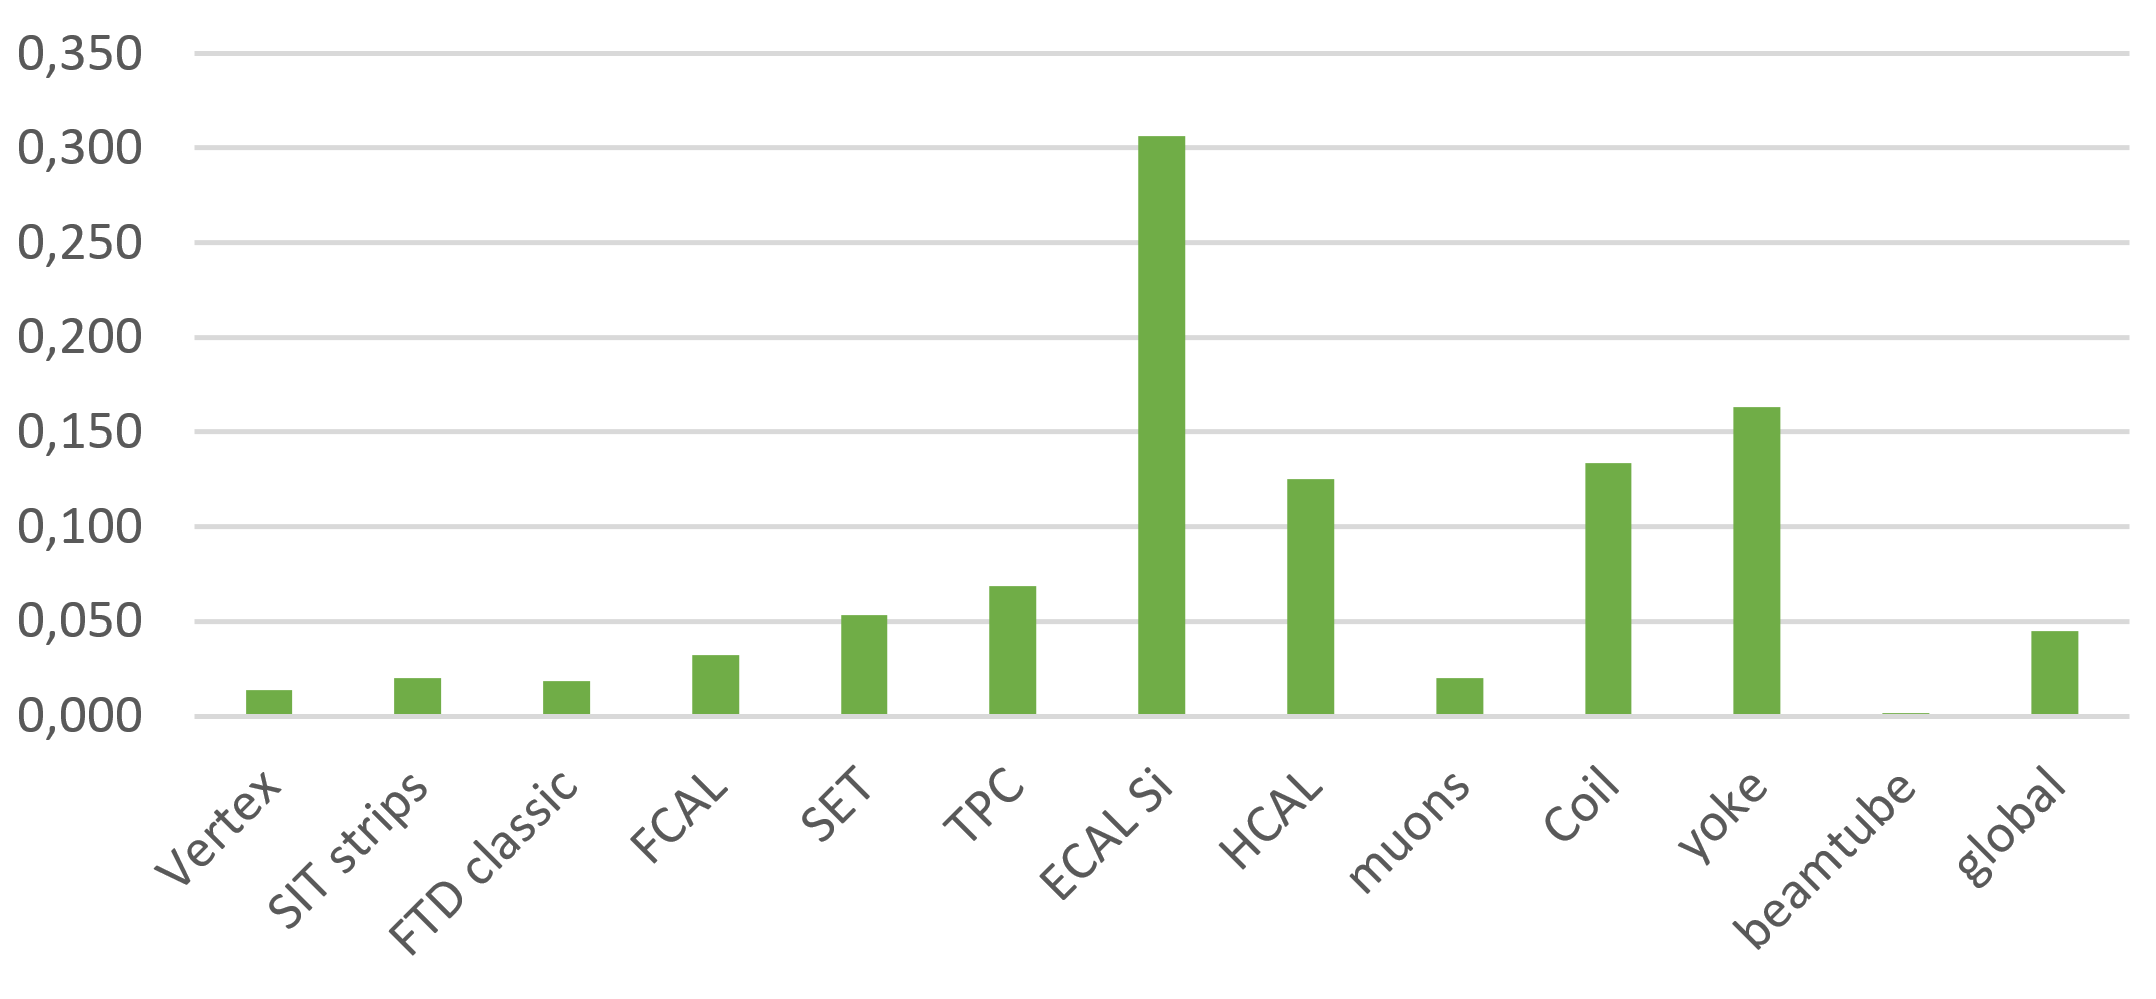
\includegraphics[width=0.8\hsize]{Costing/Small_cost_sharing.PNG}
\caption{ILD cost sharing in the small (26) model. \textit{The 30-layers baseline option should be shown instead. Empty FTD to be corrected.}}
\label{Costing:Small_cost_sharing}
\end{figure}

When comparing the updated estimations to the DBD it should be reminded that the DBD estimations did not include in house manpower and that the DBD ECAL was a mix of the Silicon and Scintillator options. 
One important message of the new estimation is that the dominant SIECAL contribution has reduced significantly using latest information from the ongoing spinoff projects of the technology, and that further reduction could be achieved by further optimizing the sampling. In the same vein the yoke cost could be reduced by 9 or even 25 MEuros depending on the stray field which can be accepted.
